% Class 5 — First research results
\documentclass[
  english,
  aspectratio=169,
]{beamer}

\usepackage{babel}
\usepackage[utf8]{inputenc}
\usepackage[T1]{fontenc}
\usepackage{booktabs}
\usepackage{hyperref}
\usepackage{tikz}

\mode<beamer>{
  \definecolor{links}{HTML}{2A1B81}
  \hypersetup{colorlinks, linkcolor=, urlcolor=links}
  \usetheme{AGH}
}

\makeatletter
\setbeamertemplate{title page}{%
  \vspace*{2.6cm}%
  \vbox{}%
  \vfill
  \hspace*{0.01\paperwidth}%
  \begingroup
  \centering
  \begin{beamercolorbox}[rounded=true,shadow=true,sep=8pt,wd=0.62\textwidth,center]{title}
    \usebeamerfont{title}\inserttitle\par
    \ifx\insertsubtitle\@empty\else
      \vskip0.25em
      {\usebeamerfont{subtitle}\usebeamercolor[fg]{subtitle}\insertsubtitle\par}%
    \fi
  \end{beamercolorbox}
  \vskip1em\par
  \begin{beamercolorbox}[sep=8pt,center]{author}
    \usebeamerfont{author}\insertauthor
  \end{beamercolorbox}
  \begin{beamercolorbox}[sep=8pt,center]{institute}
    \usebeamerfont{institute}\insertinstitute
  \end{beamercolorbox}
  \endgroup
  \vfill
}
\makeatother

\title[When Do GNNs Help?]{When Do Graph Neural Networks Help?}
\subtitle{Class 5 --- First Research Results}
\author[M.~Bro\'{s} \& M.~Burda]{%
  Micha\l{} Bro\'{s}\inst{1}
  \and
  Micha\l{} Burda\inst{1}
}
\institute[AGH]{%
  \inst{1}%
  Computational Intelligence \\
  Prof.~Adrian Horzyk \\
  AGH University of Krakow
}
\date{}

\begin{document}

\begin{frame}[plain]
  \titlepage
\end{frame}

%#####################################################################
\section{Reminder}
%#####################################################################

\begin{frame}{01~~Project reminder}
  \begin{block}{Research question}
    When do GNNs beat MLP / XGBoost, and how much edge noise
    can they survive before losing?
  \end{block}

  \begin{itemize}
    \item \textbf{H1:} on clean similar graphs GNNs win;
      after $\sim$30\% fake edges, tabular models catch up.
    \item \textbf{H2:} on mixed graphs, tabular models may win from the start.
  \end{itemize}

  \vspace{0.4em}
  \textbf{Class 5 focus:} first hypothesis test (Exp.\ A) +
  partial Exp.\ B + what failed / surprised us + next controls.
\end{frame}

\begin{frame}{02~~What we bring today}
  \begin{columns}[T]
    \begin{column}{0.48\textwidth}
      \begin{block}{Done (reproducible)}
        \begin{itemize}
          \item Data audit (Cora)
          \item Clean baseline (5 seeds)
          \item Exp.\ A edge deletion (5 seeds)
          \item Exp.\ B fake edges --- \emph{partial} (3 seeds)
        \end{itemize}
      \end{block}
    \end{column}
    \begin{column}{0.48\textwidth}
      \begin{block}{Fair protocol}
        \begin{itemize}
          \item Same Planetoid masks
          \item MLP / XGBoost / GCN
          \item Accuracy + macro-F1
          \item Saved under \texttt{RESULTS/}
        \end{itemize}
      \end{block}
    \end{column}
  \end{columns}
\end{frame}

%#####################################################################
\section{Baseline}
%#####################################################################

\begin{frame}{03~~Clean Cora baseline (reminder)}
  \begin{block}{Test accuracy --- mean $\pm$ std over 5 seeds}
    \renewcommand{\arraystretch}{1.2}
    \begin{tabular}{lcc}
      \textbf{Model} & \textbf{Test accuracy} & \textbf{Test macro-F1} \\
      \hline
      XGBoost & $0.527 \pm 0.006$ & $0.514 \pm 0.006$ \\
      MLP & $0.591 \pm 0.008$ & $0.572 \pm 0.008$ \\
      GCN & $\mathbf{0.818 \pm 0.005}$ & $\mathbf{0.806 \pm 0.005}$ \\
    \end{tabular}
  \end{block}

  \vspace{0.5em}
  Starting point of \textbf{H1}: with good (similar) connections, the graph helps
  ($\approx +23$\,pp vs MLP).
\end{frame}

%#####################################################################
\section{Experiment A}
%#####################################################################

\begin{frame}{04~~Experiment A --- delete real edges}
  \textbf{Protocol:} randomly remove undirected edges
  $0\%, 20\%, 40\%, 60\%, 80\%, 100\%$ (5 seeds).

  \begin{itemize}
    \item Tabular models ignore edges $\Rightarrow$ should stay flat
    \item GCN should fall as structure disappears
    \item At 100\% deletion GCN $\approx$ feature-only model
  \end{itemize}
\end{frame}

\begin{frame}{05~~Experiment A results}
  \begin{block}{Test accuracy (mean, 5 seeds)}
    \scriptsize
    \renewcommand{\arraystretch}{1.15}
    \begin{tabular}{lcccccc}
      \textbf{Model} & 0\% & 20\% & 40\% & 60\% & 80\% & 100\% \\
      \hline
      XGBoost & 0.527 & 0.527 & 0.527 & 0.527 & 0.527 & 0.527 \\
      MLP & 0.593 & 0.592 & 0.592 & 0.592 & 0.592 & 0.592 \\
      GCN & \textbf{0.818} & 0.793 & 0.764 & 0.726 & 0.673 & 0.594 \\
    \end{tabular}
  \end{block}

  \vspace{0.4em}
  {\small \texttt{RESULTS/expA\_cora\_summary.csv}}
\end{frame}

\begin{frame}{06~~Experiment A --- takeaways}
  \begin{itemize}
    \item MLP / XGBoost stay \textbf{flat} (control works).
    \item GCN drops smoothly: $0.82 \rightarrow 0.59$.
    \item Even after \textbf{80\%} edge removal, GCN still beats MLP
      ($0.67 > 0.59$).
    \item At \textbf{100\%}, GCN $\approx$ MLP ($0.594$ vs $0.592$).
  \end{itemize}

  \vspace{0.4em}
  \begin{block}{Hypothesis status}
    Removing real structure hurts GCN as expected, but Cora stays
    useful for GCN until almost all edges are gone.
  \end{block}
\end{frame}

%#####################################################################
\section{Experiment B}
%#####################################################################

\begin{frame}{07~~Experiment B --- add fake edges}
  \textbf{Protocol:} keep all real edges; add random non-edges
  $+0\%, 15\%, 30\%, 45\%, 60\%, 75\%$ of the real edge count.

  \begin{itemize}
    \item \textbf{H1 claim:} after $\sim$30\% fake edges, tabular overtakes GCN
    \item Status today: \textbf{partial} --- 3 seeds (0--2), same models
    \item Code: \texttt{scripts/run\_experiment\_b.py}
  \end{itemize}
\end{frame}

\begin{frame}{08~~Experiment B --- partial results (Cora)}
  \begin{block}{Test accuracy (mean over 3 seeds)}
    \scriptsize
    \renewcommand{\arraystretch}{1.15}
    \begin{tabular}{lcccccc}
      \textbf{Model} & 0\% & 15\% & 30\% & 45\% & 60\% & 75\% \\
      \hline
      XGBoost & 0.529 & 0.529 & 0.529 & 0.529 & 0.529 & 0.529 \\
      MLP & 0.586 & 0.585 & 0.585 & 0.585 & 0.585 & 0.585 \\
      GCN & \textbf{0.816} & 0.783 & 0.768 & 0.743 & 0.716 & 0.710 \\
    \end{tabular}
  \end{block}

  \vspace{0.35em}
  {\small \texttt{RESULTS/expB\_cora\_summary.csv} --- mark as partial ($n{=}3$).}
\end{frame}

\begin{frame}{09~~Experiment B --- sketch}
  \begin{center}
  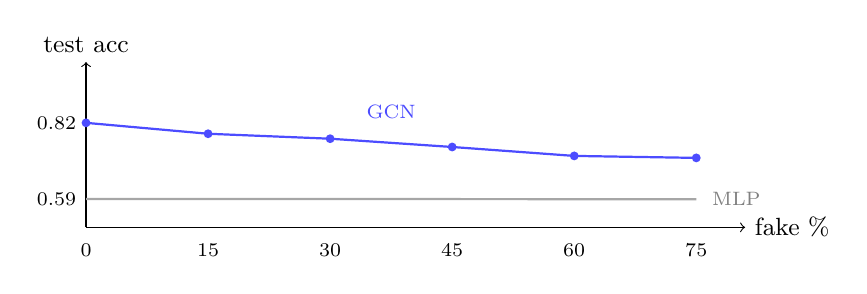
\begin{tikzpicture}[x=1.55cm,y=4.2cm]
    \draw[->] (0,0.5) -- (5.4,0.5) node[right] {\small fake \%};
    \draw[->] (0,0.5) -- (0,1.0) node[above] {\small test acc};
    % MLP flat
    \draw[thick, gray!70] (0,0.586) -- (5,0.585);
    \node[right, gray] at (5.05,0.585) {\scriptsize MLP};
    % GCN
    \draw[thick, blue!70]
      (0,0.816) -- (1,0.783) -- (2,0.768) -- (3,0.743) -- (4,0.716) -- (5,0.710);
    \foreach \x/\y in {0/0.816,1/0.783,2/0.768,3/0.743,4/0.716,5/0.710} {
      \fill[blue!70] (\x,\y) circle (1.6pt);
    }
    \node[above, blue!70] at (2.5,0.80) {\scriptsize GCN};
    \foreach \x/\lab in {0/0,1/15,2/30,3/45,4/60,5/75} {
      \node[below] at (\x,0.48) {\scriptsize \lab};
    }
    \node[left] at (0,0.816) {\scriptsize 0.82};
    \node[left] at (0,0.585) {\scriptsize 0.59};
  \end{tikzpicture}
  \end{center}

  \vspace{0.2em}
  GCN falls, but stays clearly above MLP through \textbf{+75\%} fake edges.
\end{frame}

%#####################################################################
\section{Failures}
%#####################################################################

\begin{frame}{10~~What surprised us (``failures'')}
  \begin{alertblock}{H1 breaking point $\sim$30\% --- not confirmed on Cora}
    At +30\% fake edges GCN is still $\approx 0.77$ vs MLP $\approx 0.59$.
    Even at +75\% GCN $\approx 0.71$ --- tabular does \emph{not} overtake.
  \end{alertblock}

  \begin{itemize}
    \item Cora is strongly similar ($\sim$81\% same-class neighbours)
      $\Rightarrow$ real edges still dominate under this noise protocol.
    \item Exp.\ A already showed the same pattern: advantage shrinks slowly.
    \item Negative / surprising result is useful --- we revise the claim,
      not the protocol.
  \end{itemize}
\end{frame}

\begin{frame}{11~~Updated reading of H1}
  \begin{enumerate}
    \item On clean Cora, GNN clearly helps --- \textbf{supported}.
    \item Edge deletion / fake edges degrade GCN --- \textbf{supported}.
    \item ``$\sim$30\% fake edges $\Rightarrow$ tabular wins'' ---
      \textbf{too aggressive for Cora}; revise threshold or noise type.
  \end{enumerate}

  \vspace{0.5em}
  \begin{block}{What would change our mind next}
    If GCN still wins on a \textbf{mixed} graph (Roman-empire / filtered
    Chameleon), then H2 is also weakened.
  \end{block}
\end{frame}

%#####################################################################
\section{Next}
%#####################################################################

\begin{frame}{12~~Next controlled experiments}
  \begin{enumerate}
    \item Finish Exp.\ B: extend to \textbf{5 seeds}; optional higher fake
      fractions (e.g.\ 100--200\%) or denser noise schedule.
    \item \textbf{Mixed dataset} (H2): Roman-empire or filtered Chameleon.
    \item Add \textbf{GraphSAGE} (planned main GNN for Exp.\ B); optional GAT.
    \item Class 6: ablations, uncertainty, draft of final deck.
  \end{enumerate}
\end{frame}

\begin{frame}{13~~Class 5 takeaway}
  \begin{itemize}
    \item First hypothesis test (Exp.\ A) is complete and reproducible.
    \item Partial Exp.\ B already shows GCN is \textbf{robust} to substantial
      fake-edge noise on Cora.
    \item We treat the missed $\sim$30\% breaking point as a finding,
      not a failed project.
  \end{itemize}

  \vspace{0.45em}
  \begin{block}{One sentence}
    On Cora the graph helps a lot and survives a lot of noise;
    the interesting failure mode may live on mixed graphs, not on
    mild fake-edge corruption.
  \end{block}
\end{frame}

\end{document}
